%
% File acl2014.tex
%
% Contact: koller@ling.uni-potsdam.de, yusuke@nii.ac.jp
%%
%% Based on the style files for ACL-2013, which were, in turn,
%% Based on the style files for ACL-2012, which were, in turn,
%% based on the style files for ACL-2011, which were, in turn, 
%% based on the style files for ACL-2010, which were, in turn, 
%% based on the style files for ACL-IJCNLP-2009, which were, in turn,
%% based on the style files for EACL-2009 and IJCNLP-2008...

%% Based on the style files for EACL 2006 by 
%%e.agirre@ehu.es or Sergi.Balari@uab.es
%% and that of ACL 08 by Joakim Nivre and Noah Smith

\documentclass[11pt]{article}
\usepackage{acl2015}
\usepackage{times}
\usepackage{url}
\usepackage{latexsym}
\usepackage{umoline}
\usepackage{CJKutf8}
\usepackage{expex}
\usepackage{graphicx}
\usepackage{tipa}

%\refproofing
\gathertags

\setlength\titlebox{1cm}
%\setlength\titlebox{5cm}

% You can expand the titlebox if you need extra space
% to show all the authors. Please do not make the titlebox
% smaller than 5cm (the original size); we will check this
% in the camera-ready version and ask you to change it back.

\newcommand{\zhonglogo}{\texttt{\raisebox{0.4pt}{\scriptsize[}\raisebox{-0.5pt}{|}\raisebox{0.4pt}{\scriptsize]}}}
\newcommand{\zhong}{\textsc{zhong} {\zhonglogo}}


\def\anota{\textsc{A-not-A}}

\def\aone{$A_1$}
\def\atwo{$A_2$}

%\def\argoneone{\textsc{\Overline{arg1}}}
%\def\argtwoone{\textsc{\Overline{arg2}}}
%\def\argonetwo{\textsc{\Underline{arg1}}}
%\def\argtwotwo{\textsc{\Underline{arg2}}}
\def\argoneone{$\textsc{arg1}_1$}
\def\argtwoone{$\textsc{arg2}_1$}
\def\argthreeone{$\textsc{arg3}_1$}
\def\argonetwo{$\textsc{arg1}_2$}
\def\argtwotwo{$\textsc{arg2}_2$}
\def\argthreetwo{$\textsc{arg3}_2$}

\def\lt{\ensuremath{\langle}}
\def\gt{\ensuremath{\rangle}}
\def\plus{~\ensuremath{+}~}

\newcommand{\tdl}[1]{\textit{#1}}
\newcommand{\myref}[1]{(\getref{#1})}


\title{A Constraint-based Analysis of \textsc{A-not-A} Questions in Mandarin Chinese} 


%\author{First Author \\
%  Affiliation / Address line 1 \\
%  Affiliation / Address line 2 \\
%  Affiliation / Address line 3 \\
%  {\tt email@domain} \\\And
%  Second Author \\
%  Affiliation / Address line 1 \\
%  Affiliation / Address line 2 \\
%  Affiliation / Address line 3 \\
%  {\tt email@domain} \\}

\date{}

\begin{document}
\maketitle

%\begin{abstract}
%\end{abstract}

\section{Introductory Remarks}
\label{sec:introduction}


The present study provides a constraint-based analysis of {\anota}
questions in Mandarin Chinese within the HPSG and MRS
\cite{pollard:sag:94,copestake:etal:05} framework and implements the
analysis into a computational grammar for Chinese: namely, \zhong.
Hereafter, the two components in the {\anota} structure are labelled
as {\aone} and {\atwo}, respectively.\footnote{Mandarin Chinese
  employs two negative operators such as \textit{b\`{u}} and
  \textit{m\'{e}i}, the choice of which hinges on the aspectual
  property of the verbal item that they are attached to. Due to the
  page limit, we focus on \textit{b\`{u}} herein.}


Using the {\anota} structure is one of the ways to express polar
questions in Mandarin Chinese.  The specific forms of {\anota}
questions are exemplified below.  Note that all variations presented
in \myref{exe:vnotv} convey almost the same meaning: ``Does Zhangsan
like dogs (or not like dogs)?''\footnote{Due to the page limit, this
  paper does not deal with the final type.}


{\small 
\CJK{UTF8}{gkai}{
\pex<exe:vnotv>
\a<basic>Basic: \textsc{A-not-A}\\
\begingl[glspace=.5em]
\gla 张三 喜欢 不 喜欢 狗 ?//
\glb Zh\={a}ngs\={a}n x\v{\i}huan bu x\v{\i}huan g\v{o}u ?//
\glc Zhangsan like \textsc{not} like dog \textsc{pu}//
\endgl
\a<contracted>Contracted: \textsc{A\ensuremath{^\prime}-not-A}\\
\begingl[glspace=.5em]
\gla 张三 喜 不 喜欢 狗 ?//
\glb Zh\={a}ngs\={a}n x\v{\i}huan bu x\v{\i}huan g\v{o}u ?//
\glc Zhangsan like \textsc{not} like dog \textsc{pu}//
\endgl
\a<abab1>Phrasal: \textsc{AB-not-AB}\\
\begingl[glspace=.5em]
\gla 张三 喜欢 狗 不 喜欢 狗 ?//
\glb Zh\={a}ngs\={a}n x\v{\i}huan g\v{o}u bu x\v{\i}huan g\v{o}u ?//
\glc Zhangsan like dog \textsc{not} like dog \textsc{pu}//
\endgl
\a<abab2>Phrasal: \textsc{AB-not-A}\\
\begingl[glspace=.5em]
\gla 张三 喜欢 狗 不 喜欢 ?//
\glb Zh\={a}ngs\={a}n x\v{\i}huan g\v{o}u bu x\v{\i}huan ?//
\glc Zhangsan like dog \textsc{not} like \textsc{pu}//
\endgl
\xe}}
\vspace{-20pt}

\noindent As shown in the examples above, partial reduplication can
result in either the verb being reproduced without its complement, or
the verb being reduced to only its first character/syllable.  As
illustrated in (\getfullref{exe:vnotv.contracted}), this is not
equally applicable to both {\aone} and a {\atwo}. For {\atwo}, only
one type of partial reduplication (i.e.,\ deletion of complement) is
permitted.  The lexical types capable of behaving as a syntactic head
of predicates in Mandarin Chinese, such as verbs, adjectives, and
prepositions, can participate in the {\anota} structure
\cite{tseng:09}. Two more examples in which adjectives and
prepositions are used are provided in
(\getref{exe:anota}-\getref{exe:pnotp}).


{\small 
\CJK{UTF8}{gkai}{
\ex<exe:anota>
\begingl[glspace=.5em]
\gla 张三 高 不 高 ?//
\glb Zh\={a}ngs\={a}n g\={a}o bu g\={a}o ?//
\glc Zhangsan tall \textsc{not} tall \textsc{pu}//
\glft `Is Zhangsan tall (or not tall)?'//
\endgl
\vspace{-20pt}
\xe
\ex<exe:pnotp>
\begingl[glspace=.5em]
\gla 张三 在 不 在 家 ?//
\glb Zh\={a}ngs\={a}n z\`{a}i bu z\`{a}i ji\={a} ?//
\glc Zhangsan at \textsc{not} at home \textsc{pu}//
\glft `Is Zhangsan at home (or not at home)?'//
\endgl
\xe}}
\vspace{-20pt}





\section{Basic Constraints}
\label{sec:constraints}



\subsection{Polar Questions}
\label{ssec:polar}

In the system of expressing polar questions in Mandarin Chinese,
{\anota} questions have a sibling, in which a sentence-final particle
\textit{ma} is used (henceforth, \textsc{ma}-questions).  For example,
\myref{exe:yesno} exhibits a \textit{prima facie} similarity to
(\getfullref{exe:vnotv.basic}).

{\small 
\CJK{UTF8}{gkai}{
\ex<exe:yesno>
\begingl[glspace=.5em]
\gla 张三 喜欢 狗 吗 ?//
\glb Zh\={a}ngs\={a}n x\v{\i}huan g\v{o}u ma ?//
\glc Zhangsan like dog \textsc{ma} \textsc{pu}//
\glft `Does Zhangsan like dogs?'//
\endgl
\xe}}
\vspace{-20pt}


\noindent If these two forms of polar questions are simply
allostructures of each other, the semantic represenation should be
almost the same in order for one form to be paraphrased into the other
form. However, since there are at least three reasons for believing
that they are not equivalent, there is no necessity to represent them
in a common way.  First, they are semantically different.  When a
universal quantifier \textit{d\={o}u} appears, a scope ambiguity
happens with \textsc{ma}-questions but not with {\anota} questions, as
shown in \myref{exe:scope}.


{\small 
\CJK{UTF8}{gkai}{
\pex<exe:scope>
\a<anota>
\begingl[glspace=.5em]
\gla 他们 都 喜欢 不 喜欢 开车 ?//
\glb t\={a}men d\={o}u x\v{\i}huan bu x\v{\i}huan k\={a}ich\={e} ?//
\glc they all like \textsc{not} like drive \textsc{pu}//
\glft `Do they all like to drive?'//
\endgl
\a<yesno>
\begingl[glspace=.5em]
\gla 他们 都 喜欢 开车 吗 ?//
\glb t\={a}men d\={o}u x\v{\i}huan k\={a}ich\={e} ma ?//
\glc they all like drive \textsc{ma} \textsc{pu}//
\glft `Do they all like to drive?' or // 
      `Do all of them like to drive?'
\endgl
\xe}}
\vspace{-20pt}

\noindent Second, they are pragmatically different. While the asker in
\textsc{ma}-questions has a stance to the expressed preposition
(e.g.,\ confirmation or denial), the asker in {\anota} questions does
not \cite{liing:14}. Hence, the two types of polar questions are not
necessarily interchangable. Third, they differ in terms of information
structure. In \textsc{ma}-questions, focus can be assigned to any
constitunet. For instance, in \myref{exe:yesno}, either the subject,
the object, or the verb can be evaluated as containing focus. By
contrasnt, {\anota} does not signal focus to any other elements but
the structure itself. In other words, {\anota} always bears focus
(i.e.,\ predicate focus).


\subsection{Headedness}
\label{ssec:head}



\subsection{Character}
\label{ssec:char}



{\small 
\ex\deftagex{avm:vjp}
\vspace{-10pt}
\newline
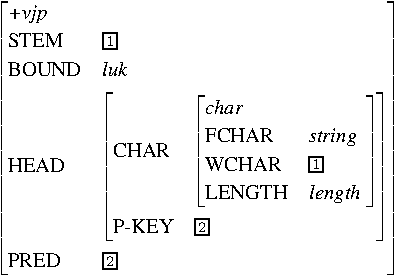
\includegraphics[scale=.8]{pdf/vjp.pdf}
\xe}
\vspace{-20pt}



{\small 
\pex<avm:xihuan>
\a<xi>
\vspace{-10pt}
\newline
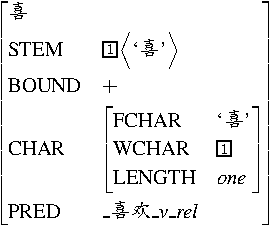
\includegraphics[scale=.8]{pdf/xi.pdf}
\a<xihuan>
\vspace{-10pt}
\newline
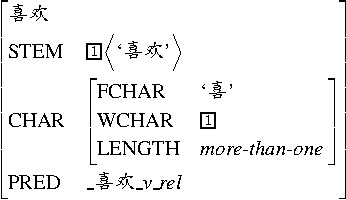
\includegraphics[scale=.8]{pdf/xihuan.pdf}
\xe}
\vspace{-20pt}





\subsection{Co-occurring Constraints}
\label{ssec:cooccurring}





Modifiability


Sentence-final Particles


\textsc{le-zhe-guo}




\section{Different Forms of {\anota} Questions}
\label{sec:forms}



\subsection{\textsc{A-not-A}}
\label{ssec:basic}



\subsection{\textsc{A\ensuremath{^\prime}-not-A}}
\label{ssec:contracted}



\subsection{\textsc{AB-not-AB}}
\label{ssec:phrasal}




\section{Implementation}
\label{sec:implemetation}


\section{Evaluation}
\label{sec:evaluation}

gTest 
pyDelphin


HELD-OUT
TEST



%\section{Conclusion}
%\label{sec:conclusion}






\bibliographystyle{acl}
\bibliography{sanghounsong}



\end{document}
